\chapter{Current Measurement For SoC Estimation}\label{ch:Current_Measurement}
SoC is the most crucial parameter of the battery to estimate in the BMS. In the deal case, the SoC of the battery has to be measured continuously, well which is not feasible since we have a measuring setup (sensors ) we need to discretize the time and, measure how much current flows through the battery to estimate the soc. To be precise in the current measure to estimate battery soc we need to account for all currents that flow in and outwards from the battery. In the active balancing setup, we have a minimum of three currents that need to be synchronized to estimate the battery soc, DC/DC converter input and output currents, and battery pack charging and discharging current. In an integrated circuit solution current measuring is very easy by designing all the sensors operating with a master clock and reading by an internal bus. Since the project is at a discrete solution level we have several current sensors associated with reading the currents. The following sections elaborate on a competitive solution for current reading and its usage in the project.
\section{Current Sensing}
To address the difficulties of creating an accurate current-measurement circuit for cost-effective applications, designers have a variety of choices at their disposal. The best flexibility is provided by using general-purpose operational amplifiers (op amps) or analog-to-digital converters (ADCs), they could be standalone or embedded in a microcontroller (MCU). While also leveraging a wide range of tailored components that are specifically made for current sensing but also address challenges in a specific way \cite{TI_Current_Sensing}.
Shunt resistors(Kelvin method) and/or hall sensors are the two methods more widely used methods in automotive BMS applications to measure the battery pack current(Charging/Discharging and Balancing current). The integrated solutions for measuring current is more preferable, to secure the space and power constraints in automotive applications. The following sections will give more insights into the current sense methods.

\section{Hall Effect Current Sensors }
"The Hall effect is the creation of a voltage difference (the Hall voltage) across an electrical conductor that is transverse to an applied magnetic field perpendicular to the current and an electric current in the conductor". Well, that is a bit of a more scientific and deep mathematical explanation of the Hall effect. If I take a little leverage to explain the Hall effect in the nomenclature The Current flow in the conductor causes to induce magnetic flux inside the magnetic core, these fluxes also turn out a small potential, which can be called hall voltage. The Hall voltage dropped across the coil (Magnetic) is directionally proportional to the current flowing in the conductor.
A galvanically isolated Hall effect current sensor capable of DC or AC measurement with high accuracy, excellent linearity, and temperature stability\cite{TI_Hall_Current_Sensing_TMCS1107}.
Let us explore hall sensors with some typical examples in the BMS such as the TMCS1107xx \cite{TI_Hall_Current_Sensing_TMCS1107} series from the TI are the most popular and competitive galvanic solutions for measuring the current.

\subsection{TMCS1107xx Sensors :}
The TMCS1107-Q1 is a galvanically isolated Hall effect current sensor with high accuracy, great linearity, and temperature stability for measuring DC or AC currents. A signal chain with low drift and temperature compensation offers a $3\%$ full-scale error over the device temperature range.\\
A magnetic field is created by the input current flowing through an internal 1.8-m conductor, which is monitored by an integrated Hall-effect sensor. This topology reduces design complexity and does away with external concentrators. Reduced conductor resistance decreases thermal and power loss. A 420-V lifetime working voltage and a 3-kV RMS minimal isolation between the current path and circuitry are provided by inherent galvanic insulation. Transient immunity and high common-mode rejection are made possible by integrated electrical shielding. \\
The output voltage is proportional to the input current. Fixed sensitivity minimizes ratiometry errors and enhances supply noise rejection, enabling the TMCS1107-Q1 to run from a single 3-V to 5.5-V power supply. When current enters the positive input pin, it is regarded as having a positive polarity. There are options for both unidirectional and bidirectional sensing.\\
\begin{figure}[h]
	\centering
	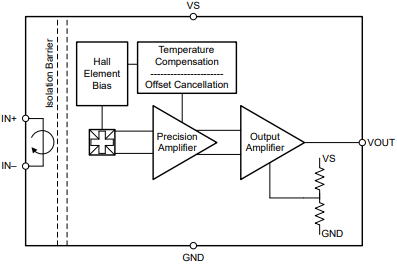
\includegraphics[width=0.6\textwidth]{Chap05/Figures/TMCS1107_HallSensor.PNG}
	\caption{TMCS1107xx Hall sensor Block diagram} 
	\label{fig:TMCS1107xx Hall sensor Block diagram}
\end{figure}
Input current to the TMCS1107-Q1 passes through the isolated side of the package lead frame through the
IN+ and IN– pins. The current flow through the package generates a magnetic field that is proportional to the
input current and measured by a galvanically isolated, precision, Hall sensor IC. As a result of the electrostatic
shielding on the Hall, sensor die, only the magnetic field generated by the input current is measured, thus limiting
input voltage switching pass-through to the circuitry\cite{TI_Hall_Current_Sensing_TMCS1107}.

\section{Shunt Resistors for Battery Current Measurement}
Sensing the voltage drop across a shunt or current-sense resistor \ref{fig:INA_high_side_currentsense} to determine the current in the most typical way. It is necessary to look at the parametric values of both the resistor and current-sense amplifier to obtain a very precise measurement of the current.
Accuracy loss must be prevented by carefully planning the connections between the current-sense amplifier and the resistor.
\begin{figure}[h]
	\centering
	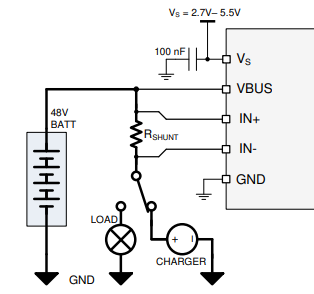
\includegraphics[width=0.4\textwidth]{Chap05/Figures/INA_high_side_currentsense.PNG}
	\caption{ INA238 High-Side Shunt Current Sensing} 
	\label{fig:INA_high_side_currentsense}
\end{figure}

INA2XX series shunt current sensors are the most competitive solution offered by TI to measure the high-side and low-side shunt current with high precision. INA238 is used in this project to measure the shunt current, bus voltage, and several other parameters. Section \ref{sec:INA238} will talk extensively about the INA238 and the features offered by the sensor to synchronize current measurements for BMS application.
\section{INA238/INA2xx}\label{sec:INA238}
The INA238 is a 16-bit delta-sigma ADC with an ultra-precise digital power monitor that is made primarily for current-sensing applications. With a common-mode voltage support range of -0.3 V to +85 V, the device can measure a full-scale differential input of $\pm$163.84 mV or $\pm$40.96 mV via a resistive shunt sensing element.
The INA238 does the necessary calculations in the background while reporting current, bus voltage, temperature, and power. The embedded temperature sensor is useful for tracking the system's ambient temperature and has a die temperature measurement accuracy of 1°C.

The INA238 can be utilized in accurate systems without undergoing multi-temperature calibration during production thanks to its low offset and gain drift design. Additionally, a wide dynamic range is provided without considerable power dissipation losses on the sensing shunt element thanks to the extremely low offset voltage and noise. This enables use in A to kA sensing applications. Due to the device's low input bias current, bigger current-sense resistors can be used, resulting in precise current readings in the micro-amp range.
The device supports samples averaging from 1x to 1024x and adjustable ADC conversion durations from 50$\mu$ s to 4.12 ms, which further reduces noise in the measured data.

\begin{figure}[h]
	\centering
	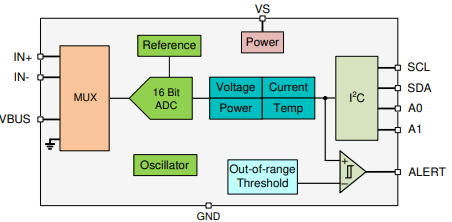
\includegraphics[width=0.6\textwidth]{Chap05/Figures/INA238_Simplified_Block_diagram.PNG}
	\label{fig:INA238_Simplified_Block_diagram}
	\caption{INA238 Simplified Block diagram \cite{INA238_User_Datasheet}}
\end{figure}

The INA238 has a multifunctional, open-drain ALERT output pin that can be utilized to report various problems or as a sign that the ADC conversion is finished while the device is functioning in both triggered and continuous conversion mode. Every time an output value under continuous monitoring exceeds its corresponding out-of-range threshold, the diagnostics mentioned in Table 7 in the user datasheet of INA238 \cite{INA238_User_Datasheet}  can be transmitted via the ALERT pin.

% \begin{table}[h]
%     \centering
%     \begin{tabular}{|l|l|l|}
%     \hline
% 		INA238 DIAGNOSTIC & STATUS BIT ALRT REGISTER (RO) & OUT-OF-RANGE THRESHOLD REGISTER (R/W)  \\ \hline
%         Shunt Under Voltage Limit & SHNTUL & SUVL\\ \hline
%         Shunt Over Voltage Limit & SHNTOL & SOVL \\ \hline
%         Bus Voltage Over-Limit & BUSOL & BOVL \\ \hline
%         Bus Voltage Under-Limit & BUSUL & BUVL \\ \hline
%         Temperature Over-Limit & TMPOL & TEMP\_LIMIT \\ \hline
%         Power Over-Limit & POL & PWR\_LIMIT & 0x7FFF H \\ \hline
%     \end{tabular}
% \end{table}

The diagnosis that prompted the ALERT pin can be identified by reading the DIAG ALRT register. In addition to configuring some ALERT pin functions, this register, which is depicted in Table 7 (user datasheet of INA238 \cite{INA238_User_Datasheet}), is also utilized to monitor other related diagnostics.

\begin{itemize}
	\item Alert latch enables — In the event that the ALERT pin is activated, this feature will maintain the pin's value even after all diagnostic circumstances have been resolved. The status of the ALERT pin is reset by reading the DIAG ALRT register. By setting the ALATCH bit, this function is made available.
	\item Conversion ready enable —  When an ADC conversion is finished and the output values are prepared to be received through the digital interface, the CONVERTION READY ENABLE signal instructs the ALERT pin to assert. Setting the CNVR bit enables this feature. Regardless of the CNVR bit set, the conversion completed events can also be read through the CNVRF bit.
	\item Alert comparison on averaged output — Enables comparison of the out-of-range threshold value to the ADC's averaged data values. Comparing the output data to the out-of-range threshold, this aids in further removing noise from the data to prevent false alarms brought on by noise. However, because of the time required for averaging, the diagnosis will be postponed. Setting the SLOWALERT bit activates this feature.
	\item Alert polarity — Allows the device to flip the ALERT pin's active state. Keep in mind that the ALERT pin is an open-drain output that requires a resistor to be pulled up. The APOL control bit can be used to change the ALERT pin's default active-low function to an active-high one.
\end{itemize}

Other diagnostic features that the ALERT pin does not report but which can be accessed by checking the DIAG ALRT register include:

\begin{itemize}
	\item Math overflow — The MATHOF bit indicates when an arithmetic operation has resulted in an internal register overflow, which is reported.
	\item Memory status — The MEMSTAT bit, which monitors the non-volatile trim memory of the device, indicates the memory status. When the gadget is functioning properly, this bit should always be set to '1'.
\end{itemize}

The ALERT pin becomes a multifunctional reporting output when set up to report the ADC conversion complete event. In the example shown in Figure \ref{fig:INA238_multi_alert}, the INA238 device reports ADC conversion complete events while also experiencing shunt over-voltage (over current), bus under voltage, over temperature, and overpower limit events.

\begin{figure}
	\centering
	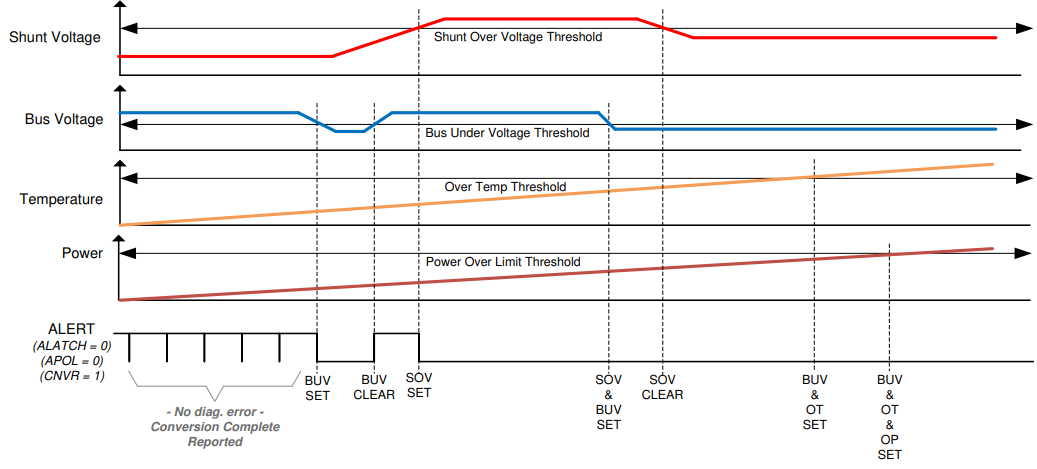
\includegraphics[width=0.8\textwidth]{Chap05/Figures/INA238_multi_alert.PNG}
	\caption{INA238 Multi-Alert Configuration}
	\label{fig:INA238_multi_alert}
\end{figure}
\section{Current Measurements Synchronization}
Section \ref{sec:INA238} described the very detailed view of INA238/INA2xx sensors, the essence of explaining INA is the most competitive solution for current measurements and it is the main pillar in this project to acquire current measurements and other several measurements(Shunt Voltage, Bus Voltage, ALERT). Among all measurements synchronizing the current measurements is the nail hitting. The following sections will brief different approaches to synchronize the current measurements.

\subsection{Simultaneous Write and Sequential Read :}
Thanks to the INA238/INA2xx multi-addressing functionality \cite[p.18]{INA238_User_Datasheet}, INA operates through I2C and the address of the INA can be configured by address lines A0 and A1 pulling to Vdd or GND. Figure \ref{fig:INA2xx_Simultaneous_Write_and_Sequential_Read}shows the Simultaneous Write and Sequential Read approach. Configure all the INAs (Write Control register) simultaneously by keeping all the INA addresses the same. Address configuration can be done, by the controller. As soon as write is done all the INAs start current acquisitions and report measurements at the same instant. For reading the current measurements, configure sensor address lines to different addresses(for instance 0x40,0x41,0x44,0x44, and so on) and read current measurements sequentially from each  INA.

\begin{figure}
    \centering
    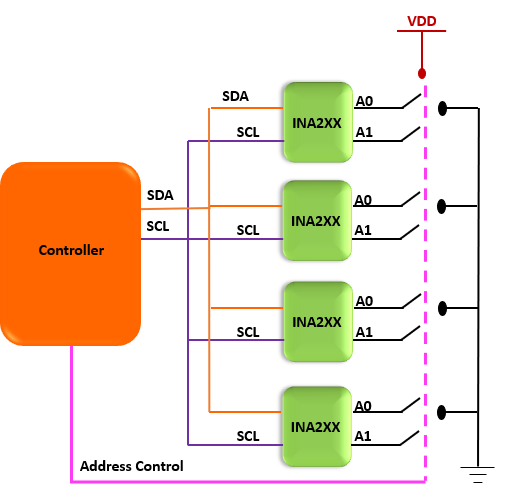
\includegraphics[width=0.4\textwidth]{Chap05/Figures/INA_MultiWrite.PNG}
    \caption{INA2xx Simultaneous Write and Sequential Read}
    \label{fig:INA2xx_Simultaneous_Write_and_Sequential_Read}
\end{figure}

"Simultaneous Write and Sequential Read" \ref{fig:INA2xx_Simultaneous_Write_and_Sequential_Read} approaches are reliable only for low precision and sequential data storage applications. SoC estimation is dealing with real-time current flowing in the battery, let's say a case where we write all sensors at the same time parallelly by considering the acknowledgment but this acknowledge could be sent by any one of the sensors if any one sensor dropped in between writing the data (configuring) controller can not differentiate. The controller only gets to know the sensor is not configured or dropped after it samples the first current data. Unfortunately, by that time the battery balancing might have already started if we do not receive current measurement data from anyone's sensor we might be in deep trouble. Simultaneous Write and Sequential Read are simple to implement but it is not robust and reliable for BMS applications.

\subsection{Synchronizing by Delayed Measurements  }
Depending on the MODE bits that have been specified and set in the ADC CONFIG register, the INA238 can measure the shunt voltage, bus voltage, die temperature, or any combination of these. This enables the user to further tune the monitoring function to meet the demands of the particular application by choosing modes to convert simply the shunt voltage or bus voltage.
\begin{figure}
    \centering
    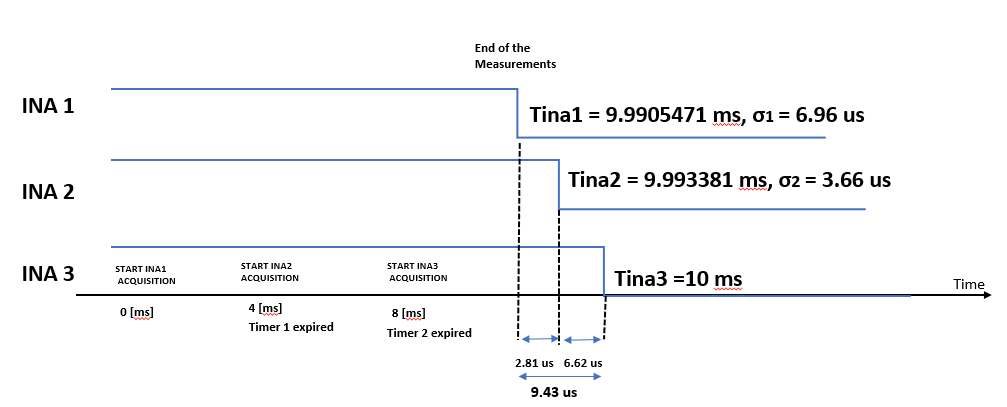
\includegraphics[width=0.9\textwidth]{Chap05/Figures/INA_synchronization_alert.PNG}
    \caption{INA2xx Delayed Synchronization}
    \label{fig:INA_synchronization_alert}
\end{figure}

The INA238 conversion can be delayed to synchronize with other system components by setting the CONVDLY bits in the CONFIG register to a value between 0 (no delay) and 510 ms. The conversion delay resolution in programming is 2 ms. By default, the conversion delay is set to 0.As soon as the measurement conversion is complete the INA2xx ALERT pin asserts. Figure \ref{fig:INA_synchronization_alert} shows synchronizing the 3 sensors by writing the sequential delay for instance first sensor has a conversion delay of 2ms subsequently adding other sensors' conversion delay (INA1 delay = INA2 delay + INA3 delay + 2ms ). At the end of the 10ms all the sensors sample at the same time, finish the conversion and assert the alert pin.  As soon as the ALERT is asserted the controller interrupts will trigger and the controller will read the data from the sensors sequentially. The point here is not reading the data sequentially or parallel important is all the sensors must sample the current at the same instance time.

\paragraph{Implementation of Synchronizing by Delayed Measurements Algorithm:}\label{sec:INA2XX_synch_delayed_method}
\begin{itemize}
    \item Send to three INAs: the config alert command (bit 14, register Bh) and sets the CONVDLY (bits 13-6 register 0h), which is the delay for initial ADC conversion. ​
    \item When START ACQUISITION command is sent, the INA waits the time specified by CONVDLY ​before starting the conversion.​
    \item CONVDLY INA 1 = 10 ms, ​CONVDLY INA 2 = 6 ms, ​CONVDLY INA 3 = 2 ms​
    \item Two Timers are used to send the start acquisition command: Timer 1 = 4ms, Timer 2 = 4ms​
    \item As two timers finish writing controller wait for ALERT interrupt to read data from sensors
\end{itemize}

Figure \ref{fig:INA_synchronization_alert} shows the three INAs synchronize current measurement current, each INA triggered with a different delay to acquire data at the end of 10ms all the INAs are asserted alert signals. The sque of the ALERT of the INAs is quite impressive because they have responded with arround 10us of sque.

So on and so forth the above sections briefed about the current sensor, features, and synchronizing methods. This section will put a more detailed view of one of the current measurement applications from BMS architecture, Power analyzer emulation, and current measurement synchronization.

\section{Balancing Current Measurement}

As discussed in chapter \ref{ch:Architecture_Active_Balancing_BMS} active balancing architecture \ref{fig:BMS Architecture}the controller will operate the DC/DC converter either in buck or boost mode depending on the unbalanced node. The output current of the DC/DC converter is the total balancing current that needs to flow from the battery node to the pack or vice versa. DC/DC converter input and output both have the shunt resistor \ref{fig:BMS Architecture} where INAs are coupled with them to measure the current. 
All the currents in the architecture \ref{fig:BMS Architecture} are measured with the power analyzer setup as briefed in chapter \ref{fig:Battery_Pack_modeling_Architec},\ref{algo:PowerAnalyzer_Modeling}(Measurement view), and all the INAs synchronized with the "INAs delayed measurement algorithm" approach as mentioned in section \ref{sec:INA2XX_synch_delayed_method}. Though, we have several currents(Charging/Discharging TOP and bottom current, DC/DC converter low and high side currents) to talk about in the architecture \ref{fig:BMS Architecture} I would like to stress the DC/DC output current more! \ref{fig:Battery_Balancing_Current}. 
Because the output current of the DC/DC converter is the balancing current that can flow from the battery node to the battery pack or vice versa, which is one of the main currents that determine the battery SOC(charging and discharging excluded in this example). 
As the balancing current reaches the threshold current (shunt current threshold set by the user Figure \ref{fig:Battery_Balancing_Current}) ALERT will be asserted by the sensor (Section \ref{sec:INA238})  and the controller will monitor the DC/DC output shunt resistor current sensor and drop the balancing current below the threshold and maintains the same current until the balancing timer period ends. 

\begin{figure}
    \centering
    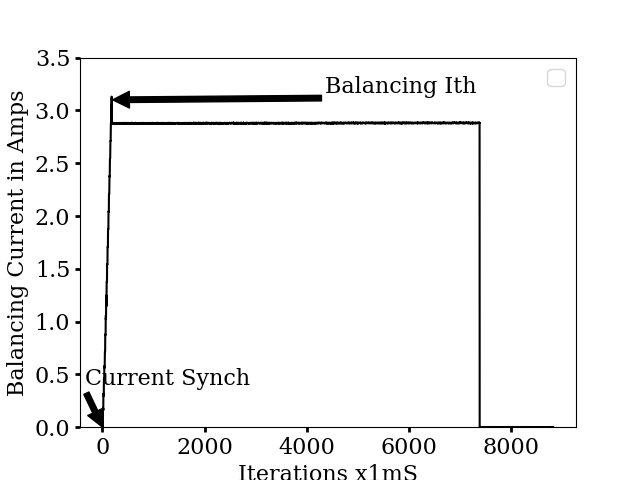
\includegraphics[width=0.6\textwidth]{Chap05/Figures/ShuntCurrent.png}
    \caption{Battery Balancing Current}
    \label{fig:Battery_Balancing_Current}
\end{figure}

\section{Summery of Chapter \ref{ch:Current_Measurement}}

Chapter \ref{ch:Current_Measurement} provided me an opportunity to explore different kinds of current measuring sensors for the BMS application and synchronize current measurements, after a deep analysis finally we landed with INA2xx series sensors. In section \ref{sec:INA238}, I took the advantage of explaining deeply about the current sensor, because most of the measurements and decisions are taken by the controller depend on the current sensor during the balancing for instance balancing current, balancing node voltage, balancing current thresholds, bus voltage threshold, and so on. INA current sensor ALERT signal configuration gave an extensive chance to explore the synchronization of the current measurement estimating the battery SoC. Battery balancing current results (Figure \ref{fig:Battery_Balancing_Current}) measured through the power analyzer model will interpolate the BMS architecture discussed in chapter \ref{ch:Architecture_Active_Balancing_BMS} to the Powel Analyzer architecture in chapter 4. This chapter can also become the fundamental pillar for chapter 5 to estimate the SOC with several algorithms (synchronization with Delayed Measurements and Parallel Wite; Sequential Read).